\documentclass{templateNote}
\usepackage{tcolorbox}
\usepackage{xcolor}
\usepackage{amssymb}
\usepackage{pgfplots}
\usepackage{hyperref}

\pgfplotsset{compat=1.18}

\newcommand{\destacar}[1]{ \colorbox{yellow}{#1}}

\begin{document}
\imagenlogoU{img/LogoElNube.png}
\linklogoU{https://github.com/MarceloPazPezo}
\imagenlogoD{img/LogoNGM.png}
\linklogoD{https://github.com/NicoxlkboUni}
\linkDoc{https://github.com/MarceloPazPezo/MyRepo/blob/main/Icinf/Semestre\%206/Economia\%201/Test\%202/Apunte\%20Test\%202.pdf}
\universidad{Universidad del Bío-Bío}
\titulo{Apunte Test 2} % Titulo
\asignatura{Economia 1} % Asignatura
\autor{
    % \indent
    Nicolas \textsc{Gomez}
    \quad
    Marcelo \textsc{Paz}
}
\portada
\margenes % Crear márgenes

\section{Importante}
\begin{itemize}
    \item \textbf{Excedente del consumidor:} Es la diferencia entre el precio que está dispuesto a pagar el consumidor y el precio que realmente paga.
    
    Para calcularlo en rectas se puede usar la siguiente formula:
    \begin{align*}
        EC = \begin{cases}
                \displaystyle \frac{(P_{max} - P_{eq}) \cdot (Q_{eq} - Q_{min})}{2} \qquad \textbf{, en rectas}\\
                \displaystyle \int_{Q_{min}}^{Q_{eq}}{(Q(x)^{d} - P_{eq})dx} \qquad \textbf{, en curvas}
            \end{cases}
    \end{align*}
    \begin{figure}[H]
        \centering
        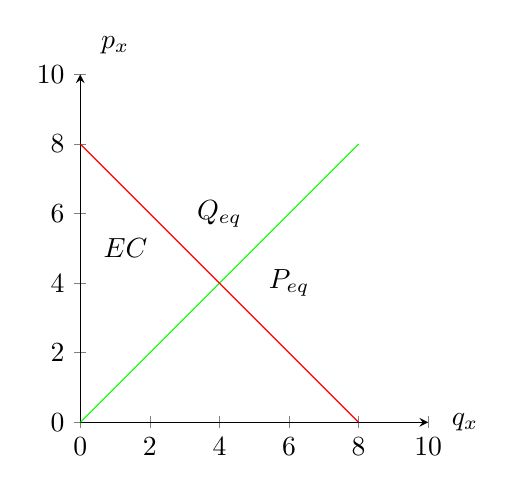
\begin{tikzpicture}
            \begin{axis}[ 
                axis lines = left,
                xlabel style={at={(rel axis cs:1.04,0)}, anchor=west},
                ylabel style={rotate =-90 ,at={(rel axis cs:0.10,1.03)}, anchor=south},
                xmax = 10,
                ymax = 10,
                height = 6cm,
                width = 6cm,
                xmin = 0,
                ymin = 0,
                xlabel = $q_x$,
                ylabel = $p_x$,
            ]

            \filldraw[fill=red!10!white, draw=none] (0,80) -- (40,40) -- (0,40) -- cycle;
            
            \addplot [
                domain=0:8, 
                samples=100, 
                color=green,
            ]
            {x};
            
            \addplot [
                domain=0:8, 
                samples=100, 
                color=red,
            ]
            {8-x};

            \node[fill=none] at (axis cs: 1.3, 5) {$EC$};
            \node[fill=none] at (axis cs: 6, 4) {$P_{eq}$};
            \node[fill=none] at (axis cs: 4, 6) {$Q_{eq}$};
            \draw [dashed] (0,40) -- (50,40);
            \draw [dashed] (40,0) -- (40,50);

            \end{axis}
        \end{tikzpicture}
        \caption{Excedente del Consumidor}
        \begin{align*}
            EC = \begin{cases}
                     \displaystyle \frac{(8 - 4) \cdot (4 - 0)}{2} = 8 \\
                    \int_{0}^{4}{(8-x-4)}dx = 4x - \frac{x^2}{2} \Big|_{0}^{4} = 8 
                \end{cases}
        \end{align*}
    \end{figure}
    \begin{itemize}
        \item \destacar{Area entre la curva de demanda y el precio de equilibrio.}
        \item Cuando aumenta el precio de equilibrio el excedente del consumidor disminuye y si disminuye el precio de
        equilibrio lo contrario.
    \end{itemize}


    \newpage
    \item \textbf{Excedente del productor:} Es la diferencia entre el precio que está dispuesto a vender el productor y el precio que realmente vende.
    \begin{align*}
        EP = \begin{cases}
                \displaystyle \frac{(P_{eq} - P_{min}) \cdot (Q_{eq} - Q_{min})}{2} \qquad \textbf{, en rectas}\\
                \displaystyle \int_{Q_{min}}^{Q_{eq}}{(P_{eq}-Q(x)^{s})dx} \qquad \textbf{, en curvas}
            \end{cases}
    \end{align*}

    \begin{figure}[H]
        \centering
        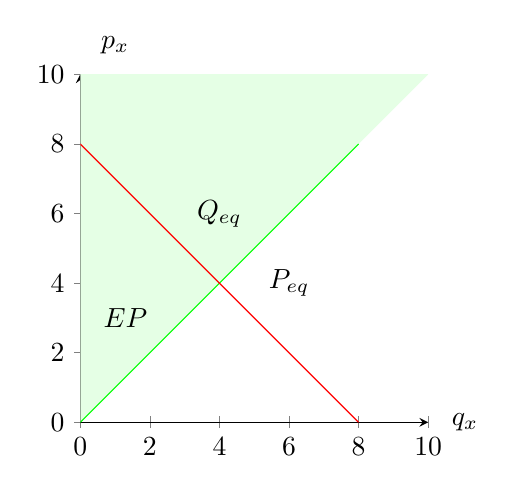
\begin{tikzpicture}
            \begin{axis}[ 
                axis lines = left,
                xlabel style={at={(rel axis cs:1.04,0)}, anchor=west},
                ylabel style={rotate =-90 ,at={(rel axis cs:0.10,1.03)}, anchor=south},
                xmax = 10,
                ymax = 10,
                height = 6cm,
                width = 6cm,
                xmin = 0,
                ymin = 0,
                xlabel = $q_x$,
                ylabel = $p_x$,
            ]

            \filldraw[fill=green!10!white, draw=none] (0,0) -- (40,40) -- (0,40) -- cycle;
            
            \addplot [
                domain=0:8, 
                samples=100, 
                color=green,
            ]
            {x};
            
            \addplot [
                domain=0:8, 
                samples=100, 
                color=red,
            ]
            {8-x};

            \node[fill=none] at (axis cs: 1.3, 3) {$EP$};
            \node[fill=none] at (axis cs: 6, 4) {$P_{eq}$};
            \node[fill=none] at (axis cs: 4, 6) {$Q_{eq}$};
            \draw [dashed] (0,40) -- (50,40);
            \draw [dashed] (40,0) -- (40,50);

            \end{axis}
        \end{tikzpicture}
        \caption{Excedente del Productor}
        \begin{align*}
            EP = \begin{cases}
                    \displaystyle \frac{(8 - 4) \cdot (4 - 0)}{2} = 8 \\
                    \displaystyle \int_{0}^{4}{(4-x)}dx = 4x - \frac{x^2}{2} \Big|_{0}^{4} = 8
                \end{cases}
        \end{align*}
    \end{figure}
    \begin{itemize}
        \item \destacar{Area entre el precio de equilibrio y la curva de oferta.}
    \end{itemize}

    \item \textbf{Perdida/Ganancia en el excedente:} se puede calcular como la diferencia entre el
    excedente original y el actual.

    \item \textbf{Oferta Laboral:} Se modela utilizando restricciones presupuestarias y curvas de
    indiferencia.
    
    La restricción presupuestaria se visualiza mediante un gráfico que representa la relación entre el
    consumo y las horas. A medida que las horas se alejan del punto cero, se incrementan las horas
    de ocio, y a medida que se acercan, aumentan las horas de trabajo. Este último comportamiento
    influye en el aumento del consumo.
    
    El óptimo ocio-consumo está dado cuando la curva de indiferencia valorada por los individuos
    es tangente a la restricción de presupuesto equivalente a la pendiente de su gráfica.

    Las curvas de oferta laboral pueden tomar cualquier forma.

    El impuesto al ingreso afecta directamente al consumo reduciendo la capacidad de compra del
    individuo.

    \newpage
    Algebraicamente:
    \begin{align*}
        \text{Restricción presupuestaria:} \qquad & C = w \cdot (T - n) \\
        \text{Re-escrita como:} \qquad & c + w \cdot n = w \cdot T
    \end{align*}
    
    Donde,
    \begin{itemize}
        \item $C$ es el consumo.
        \item $n$ es el número de horas de ocio por semana.
        \item El precio de C es 1.
        \item $w$ es el salario. El "precio" del ocio es el salario perdido (w).
        \item El ingreso total es el valor de la dotación de tiempo, $wT$.
    \end{itemize}

    \begin{figure}[H]
        \centering
        \begin{tikzpicture}
            \begin{axis}[ 
                axis lines = left,
                xlabel style={at={(rel axis cs:1.04,0)}, anchor=west},
                ylabel style={rotate =-90 ,at={(rel axis cs:0.10,1.03)}, anchor=south},
                xmax = 178,
                ymax = 70,
                height = 8cm,
                width = 12cm,
                xmin = 0,
                ymin = 0,
                xlabel = $\text{Horas de ocio}$,
                ylabel = $\text{Consumo}$,
            ]

            \addplot [
                domain=0:168, 
                samples=100, 
                color=green,
            ]
            {60-x/2.8};

            \end{axis}
        \end{tikzpicture}
        \caption{Restricción presupuestaria}

    \end{figure}

    \item \textbf{Valoración Marginal:} Son curvas de demanda reflejan la disposición máxima a pagar por un bien especifico.

    \item \textbf{Valoración Total:} Es la suma de las valoraciones marginales (Puede limitarse a un número de
    unidades específicas). De manera general, el área bajo la curva (línea) de la demanda entre la
    primera y última unidad.
    
    \newpage
    \item \textbf{Empresas:} Organización que convierte insumos en productos:
    \begin{itemize}
        \item \textbf{Servicios de capital (K):} Insumos de larga duración.
        
        \item \textbf{Servicios laborales (L):} Horas de trabajo proporcionadas.
        
        \item \textbf{Materiales (M):} Recursos naturales y productos procesados consumidos en producción o
        implementados a un producto final.
        
        \item \textbf{Productos:} Bienes y servicios.
    \end{itemize}

    Tipos de empresas:
    \begin{itemize}
        \item \textbf{Empresas Privadas (Fines de lucro):} Propiedad de individuos que buscan ganancias.
        
        \item \textbf{Empresas Públicas:} Propiedad de gobiernos o agencias gubernamentales.
        
        \item \textbf{Empresas sin fines de lucro:} Propiedad de organizaciones no gubernamentales que no
        buscan ganancias.        
    \end{itemize}

    Las empresas privadas buscan maximizar las ganancias(diferencia entre ingresos y costos).
    \begin{itemize}
        \item \textbf{Ingreso ($IT = p \cdot q$):} Pago recibido por la venta de producto con p como el valor del
        producto y q como la cantidad vendida de este.
        
        \item \textbf{Costo ($CT$):} Lo que se paga para producir el producto.
        
        \item \textbf{Beneficio/Utilidad:} $IT - CT$
    \end{itemize}

    \item \textbf{Función de Producción:} Relación entre la cantidad de insumos y la cantidad de producto.
    \begin{align*}
        q = Q = f(L,K)
    \end{align*}
    Donde $L$ es la cantidad de trabajo y $K$ es la cantidad de capital.
    \begin{itemize}
        \item \textbf{Corto Plazo:} Periodo de tiempo en el que el capital $K$ se mantendrá constante.
        \begin{align*}
            q_{cp} = f(L, \overline{K})
        \end{align*}
        
        \item \textbf{Largo Plazo:} Todos los insumos son variables.
        \begin{align*}
            q_{lp} = f(L,K)
        \end{align*}
    \end{itemize}

    \item \textbf{Producto marginal del trabajo:} Producto adicional producido por una unidad adicional
    de trabajo.
    \begin{align*}
        PM_{g_{L}} = \frac{\partial Q}{\partial L}
    \end{align*}

    \item \textbf{Producto medio del trabajo:} Relación entre la producción y el trabajo.
    \begin{align*}
        PM_{e_{L}} = \frac{Q}{L}
    \end{align*}

    \item \textbf{Ley de rendimientos marginales decrecientes (LDRD):} Si se aumenta un insumo manteniendo
    los demás insumos y tecnologías constantes los aumentos en la producción serán menores, por lo
    que eventualmente:
    \begin{align}
        \frac{\partial PM_{g_{L}}}{\partial L} < 0
    \end{align}
    
    \item \textbf{Retornos de Escala:}
    Considere la función de producción $Q = f(L, K)$

    Se multiplica todos los factores por x y se obtiene:
    \begin{align*}
        Q = f(xL, xK) = x^{\alpha}f(L, K)
    \end{align*}
    \begin{itemize}
        \item Rendimientos \destacar{Constantes} a Escala: Si $\alpha = 1$.
        
        \item Rendimientos \destacar{Decrecientes} a Escala: Si $\alpha < 1$.
        
        \item Rendimientos \destacar{Crecientes} a Escala: Si $\alpha > 1$.
    \end{itemize}

    \item \textbf{Función de producción Cobb-Douglas:} Es una función de producción que tiene la forma:
    \begin{align*}
        Q = f(L,K) = A \cdot L^{\alpha}K^{\beta}
    \end{align*}

    \item \textbf{Isocuantas:} representa gráficamente combinaciones de trabajo y producción.
    
    Producción constante a lo largo de la curva.
    \begin{align*}
        \overline{q} = f(L,K)
    \end{align*}

    Propiedades(similares a las curvas de indiferencia):
    \begin{itemize}
        \item Cuanto más lejos esta una isocuanta del origen, mayor es el nivel de producción.
        \item Las isocuantas no se cruzan.
        \item Las isocuantas tienen pendiente negativa.
        \item Las isocuantas deben ser delgadas
    \end{itemize}

    \newpage
    Tipos:
    \begin{itemize}
        \item \textbf{Sustitución perfecta:} Cuando los insumos son perfectamente sustituibles.
        \begin{align*}
            q = K + L
        \end{align*}
        \begin{figure}[H]
            \centering
            \begin{tikzpicture}
                \begin{axis}[ 
                    axis lines = left,
                    xlabel style={at={(rel axis cs:1.04,0)}, anchor=west},
                    ylabel style={rotate =-90 ,at={(rel axis cs:0.10,1.03)}, anchor=south},
                    xmax = 6,
                    ymax = 6,
                    height = 8cm,
                    width = 8cm,
                    xmin = 0,
                    ymin = 0,
                    xlabel = $K$,
                    ylabel = $L$,
                ]
    
                \addplot [
                    domain=0:1, 
                    samples=100, 
                    color=blue,
                ]
                {1-x};

                \addplot [
                    domain=0:2, 
                    samples=100, 
                    color=blue,
                ]
                {2-x};

                \addplot [
                    domain=0:3, 
                    samples=100, 
                    color=blue,
                ]
                {3-x};

                \addplot [
                    domain=0:4, 
                    samples=100, 
                    color=blue,
                ]
                {4-x};

                \addplot [
                    domain=0:5, 
                    samples=100, 
                    color=blue,
                ]
                {5-x};
    
                \end{axis}
            \end{tikzpicture}
            \caption{Sustitución perfecta}
    
        \end{figure}

        \item \textbf{Producción fija:} Cuando la producción no depende de la cantidad de insumos.
        \begin{align*}
            q = min(K, L)
        \end{align*}
        \begin{figure}[H]
            \centering
            \begin{tikzpicture}
                \begin{axis}[ 
                    axis lines = left,
                    xlabel style={at={(rel axis cs:1.04,0)}, anchor=west},
                    ylabel style={rotate =-90 ,at={(rel axis cs:0.10,1.03)}, anchor=south},
                    xmax = 6,
                    ymax = 6,
                    height = 8cm,
                    width = 8cm,
                    xmin = 0,
                    ymin = 0,
                    xlabel = $K$,
                    ylabel = $L$,
                ]
    
                \addplot [
                    domain=1:6, 
                    samples=100, 
                    color=blue,
                ]
                {1};

                \draw[color=blue] (100,100) -- (100,600);
                
                \addplot [
                    domain=2:6, 
                    samples=100, 
                    color=blue,
                ]
                {2};

                \draw[color=blue] (200,200) -- (200,600);

                \addplot [
                    domain=3:6, 
                    samples=100, 
                    color=blue,
                ]
                {3};

                \draw[color=blue] (300,300) -- (300,600);

                \addplot [
                    domain=4:6, 
                    samples=100, 
                    color=blue,
                ]
                {4};

                \draw[color=blue] (400,400) -- (400,600);

                \addplot [
                    domain=5:6, 
                    samples=100, 
                    color=blue,
                ]
                {5};
    
                \draw[color=blue] (500,500) -- (500,600);
    
                \end{axis}
            \end{tikzpicture}
            \caption{Producción fija}
    
        \end{figure}

        \item \textbf{Convexa(Cobb-Douglas):} Cuando los insumos son complementarios.
        \begin{align*}
            q = A \cdot L^{\alpha}K^{\beta}
        \end{align*}
        \begin{figure}[H]
            \centering
            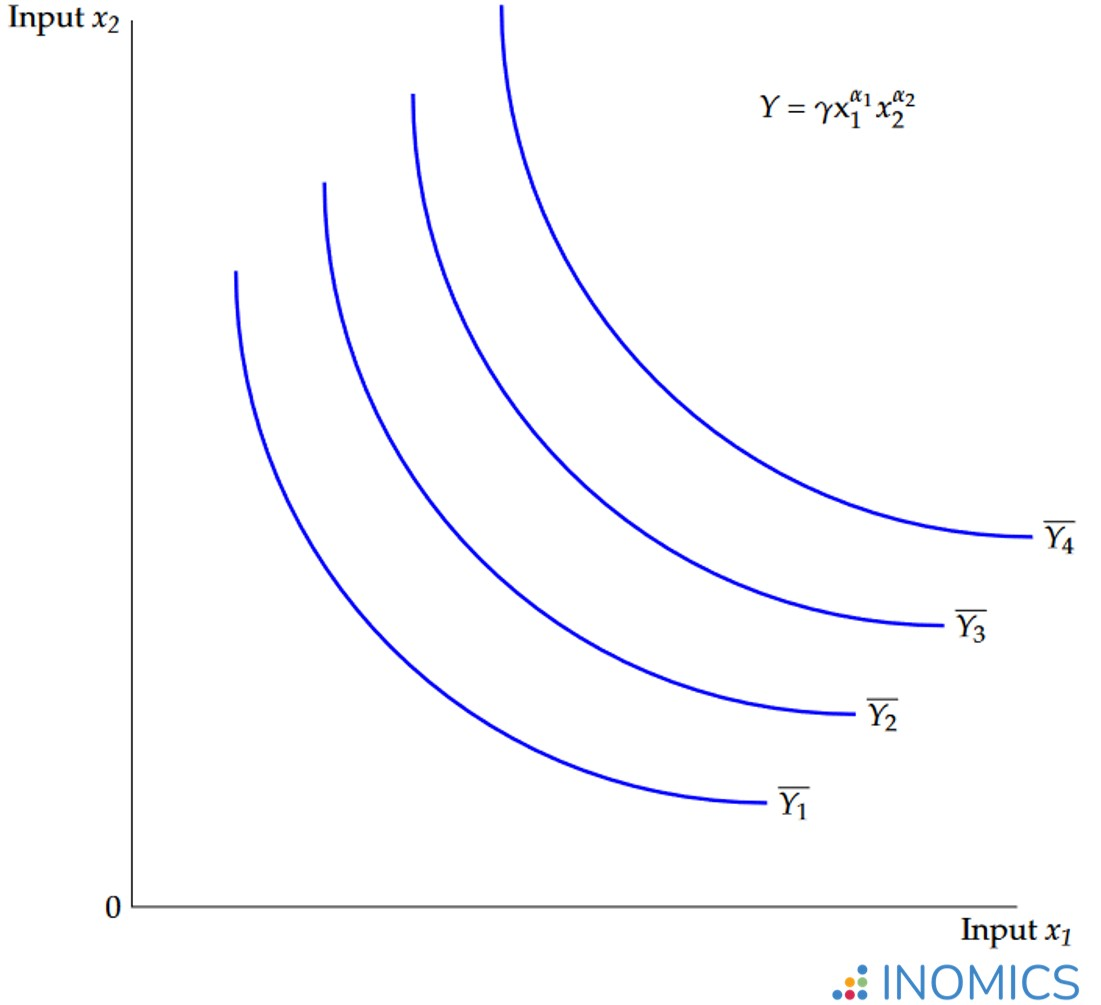
\includegraphics[width=0.5\textwidth]{img/Convexa.jpg}
            \caption{Convexa}
        \end{figure}
    \end{itemize}

    \item \textbf{Pendientes Isocuantas:} Relación marginal de sustitución (RMST) pendiente isocuanta en un punto especifico:
    \begin{align*}
        RMST = \frac{\Delta K}{\Delta L} = \frac{d K}{dL}
    \end{align*}

    Para funciones de producción:
    \begin{align*}
        RMST = \begin{cases}
            \displaystyle = \frac{dK}{dL} = - \frac{\left[\frac{\partial f(L,K)}{\partial L}\right]}{\left[\frac{\partial f(L,K)}{\partial K}\right]} = - \frac{PM_{g_{L}}}{PM_{g_{K}}} & \text{, convexa} \\
            \displaystyle = -1 & \text{, lineal} \\
            \displaystyle = \text{No esta definido} & \text{, fija} \\
        \end{cases}
    \end{align*}
    Para la función de producción fija no es posible la sustitución $PM_{g_{K}} = 0$

\end{itemize}

\newpage
\section{Ejercicios}
\subsection{Ayudantia 8}
\subsubsection{Ejercicio 1}
Función de producción:
\begin{align*}
    Q(K, L) = 1,1L^{0,3}K^{0,7}
\end{align*}

En donde K es la cantidad de capital y L es la cantidad de trabajo utilizado. Se pide:

\subitem \textbf{A)}  Calcule la productividad marginal y media del trabajo e interprete los resultados
\begin{align*}
    PM_{g_{L}} &= \frac{\partial Q}{\partial L} \\
    &= \frac{1,1 L^{0,3}K^{0,7}}{\partial L} \\
    &= 1,1 \cdot 0,3 \cdot L^{0,3 - 1}K^{0,7} \\
    &= 0,33L^{-0,7}K^{0,7} \qquad \text{Productividad Marginal del Trabajo}
\end{align*}
\begin{align*}
    PM_{e_{L}} &= \frac{Q}{L} \\
    &= \frac{1,1 L^{0,3}K^{0,7}}{L} \\
    &= 1,1 \cdot L^{0,3 - 1}K^{0,7} \\
    &= 1,1L^{-0,7}K^{0,7} \qquad \text{Productividad Media del Trabajo}
\end{align*}

Interpretación:
\begin{itemize}
    \item \destacar{Productividad Marginal del Trabajo:} Es la variación de la producción total cuando se aumenta una unidad de trabajo, manteniendo constante la cantidad de capital.
    \item \destacar{Productividad Media del Trabajo:} Es la producción total dividida por la cantidad de trabajo utilizado.
\end{itemize}

\subitem \textbf{B)} Mencionar que rendimientos de escala presenta la función de producción.
\begin{align*}
    Q(K, L) = 1,1L^{0,3}K^{0,7}
\end{align*}
\begin{align*}
    Q(2K, 2L) &= 1,1(2L)^{0,3}(2K)^{0,7} \\
    &= 1,1 \cdot 2^{0,3}L^{0,3} \cdot 2^{0,7}K^{0,7} \\
    &= 2^{0,3 + 0,7} \cdot 1,1 \cdot L^{0,3}K^{0,7} \\
    &= 2(1,1L^{0,3}K^{0,7}) \\
    &= 2Q(K, L)
\end{align*}
\begin{align*}
    \text{Rendimientos de escala:} \qquad & \text{Constante}
\end{align*}

\newpage
\subsubsection{Ejercicio 2}
Mencionar cuál es la diferencia entre la producción de corto plazo y largo plazo

\textbf{Respuesta:}
En el corto plazo generalmente $\overline{K}$ es fijo a comparación del largo plazo.


\subsubsection{Ejercicio 3}
Calcular la productividad media del capital de la siguiente función de producción:
\begin{align*}
    Q(K, L) = 1,1L^{0,3}K^{0,7}
\end{align*}
\begin{align*}
    PM_{e_{K}} &= \frac{Q}{K} \\
    &= \frac{1,1 L^{0,3}K^{0,7}}{K} \\
    &= 1,1 \cdot L^{0,3}K^{0,7 - 1} \\
    &= 1,1L^{0,3}K^{-0,3} \qquad \text{Productividad Media del Capital}
\end{align*}

\subsubsection{Ejercicio 4}
Señale Verdadero (V) o Falso (F), según corresponda:
\begin{itemize}
    \item F: Una función de producción muestra la relación entre trabajo y productos cuando la
    producción es eficiente.

    \textbf{Justificación:} Una función de producción muestra la relación entre insumos y productos cuando la producción es eficiente.

    \textbf{Copilot:} Verdadero. Una función de producción muestra la relación entre los insumos (como el trabajo) y los productos cuando la producción es eficiente. Esta función describe la cantidad máxima de producto que se puede obtener de cada combinación de insumos. Por lo tanto, sí, tu afirmación es correcta.
    
    \item V: El producto marginal del trabajo es el producto adicional producido por una unidad
    adicional de trabajo, manteniendo constantes todos los demás factores (ceteris paribus).
    
    \item F:  La función de producción es $q = f(T, K)$ la cual muestra solo la cantidad máxima de
    producción que se puede producir a partir de niveles dados de trabajo y capital.
    
    \textbf{Justificación:} La función de producción es $q = f(L, K)$.
    
    \item F: Existen dos tipos de empresas: públicas y sin fines de lucro.
    
    \textbf{Justificación:} Existen tres tipos de empresas: públicas, \destacar{privadas} y sin fines de lucro.

    \item F: La función de producción de una empresa es: $ q = 0,5 LK + 5 L^2K - 0,5 L^3K$, si el capital es fijado en $K = 20$, la producción a corto plazo será $q = 10 L + 100 L^2 - 20 L^3$
    \begin{align*}
        q &= 0,5 LK + 5 L^2K - 0,5 L^3K \\
        &= 0,5 \cdot 20 \cdot L + 5 \cdot 20 \cdot L^2 - 0,5 \cdot 20 \cdot L^3 \\
        &= 10L + 100L^2 - 10L^3
    \end{align*}
\end{itemize}

\newpage
\subsubsection{Ejercicio 5}

La función de producción de una empresa es:
\begin{align*}
    q &= 0,5 LK + 5 L^2K - 0,5 L^3K
\end{align*}

\subitem \textbf{A)}  ¿Cuál es el producto marginal del trabajo $(PM_{g_{L}})$?
\begin{align*}
    PM_{g_{L}} &= \frac{\partial Q}{\partial L} \\
    &= \frac{0,5 LK + 5 L^2K - 0,5 L^3K}{\partial L} \\
    &= 0,5K + 10LK - 1,5L^2K \qquad \text{Producto Marginal del Trabajo}
\end{align*}

\subitem \textbf{B)} ¿Cuál es el producto medio del trabajo $(PM_{g_{L}})$?
\begin{align*}
    PM_{e_{L}} &= \frac{Q}{L} \\
    &= \frac{0,5 LK + 5 L^2K - 0,5 L^3K}{L} \\
    &= 0,5K + 5LK - 0,5L^2K \qquad \text{Producto Medio del Trabajo}
\end{align*}

\end{document}